\documentclass{beamer}

\newcommand{\course}{CS 1331 Introduction to Object Oriented Programming}
\newcommand{\lesson}{{\tt Java Collections (Part 1 of 3)}}
\newcommand{\code}{http://www.cc.gatech.edu/~simpkins/teaching/gatech/cs1331/code}

\author[Chris Simpkins] 
{Christopher Simpkins \\\texttt{chris.simpkins@gatech.edu}}
\institute[Georgia Tech] % (optional, but mostly needed)

\date[CS 1331]{}


\newcommand{\course}{Introduction to Object-Oriented Programming}
\subject{\course}
\title[\lesson]{\course}
\subtitle{\lesson}

\author[CS 1331]
{Christopher Simpkins \\\texttt{chris.simpkins@gatech.edu}}
\institute[Georgia Tech]

\date[]{}

\newcommand{\link}[2]{\href{#1}{\textcolor{blue}{\underline{#2}}}}
\newcommand{\code}{http://www.cs1331.org/code}

\usepackage{colortbl}

% If you have a file called "university-logo-filename.xxx", where xxx
% is a graphic format that can be processed by latex or pdflatex,
% resp., then you can add a logo as follows:

% \pgfdeclareimage[width=0.6in]{coc-logo}{cc_2012_logo}
% \logo{\pgfuseimage{coc-logo}}

\mode<presentation>
{
  \usetheme{Berlin}
  \useoutertheme{infolines}

  % or ...

 \setbeamercovered{transparent}
  % or whatever (possibly just delete it)
}

\usepackage{tikz}
% Optional PGF libraries
\usepackage{pgflibraryarrows}
\usepackage{pgflibrarysnakes}
\usepackage{pgfplots}
\usepackage{fancybox}
\usepackage{listings}
\usepackage{hyperref}
\hypersetup{colorlinks=true,urlcolor=blue}
\usepackage[english]{babel}
% or whatever

\usepackage[latin1]{inputenc}
% or whatever

\usepackage{times}
\usepackage[T1]{fontenc}
% Or whatever. Note that the encoding and the font should match. If T1
% does not look nice, try deleting the line with the fontenc.


\usepackage{listings}

% "define" Scala
\lstdefinelanguage{scala}{
  morekeywords={abstract,case,catch,class,def,%
    do,else,extends,false,final,finally,%
    for,if,implicit,import,match,mixin,%
    new,null,object,override,package,%
    private,protected,requires,return,sealed,%
    super,this,throw,trait,true,try,%
    type,val,var,while,with,yield},
  otherkeywords={=>,<-,<\%,<:,>:,\#,@},
  sensitive=true,
  morecomment=[l]{//},
  morecomment=[n]{/*}{*/},
  morestring=[b]",
  morestring=[b]',
  morestring=[b]""",
}

\usepackage{color}
\definecolor{dkgreen}{rgb}{0,0.6,0}
\definecolor{gray}{rgb}{0.5,0.5,0.5}
\definecolor{mauve}{rgb}{0.58,0,0.82}

% Default settings for code listings
\lstset{frame=tb,
  language=scala,
  aboveskip=2mm,
  belowskip=2mm,
  showstringspaces=false,
  columns=flexible,
  basicstyle={\scriptsize\ttfamily},
  numbers=none,
  numberstyle=\tiny\color{gray},
  keywordstyle=\color{blue},
  commentstyle=\color{dkgreen},
  stringstyle=\color{mauve},
  frame=single,
  breaklines=true,
  breakatwhitespace=true,
  keepspaces=true
  %tabsize=3
}


% If you wish to uncover everything in a step-wise fashion, uncomment
% the following command: 

% \beamerdefaultoverlayspecification{<+->}


\begin{document}

\begin{frame}
  \titlepage
\end{frame}


%------------------------------------------------------------------------
\begin{frame}[fragile]{The Collections Framework}

\begin{center}
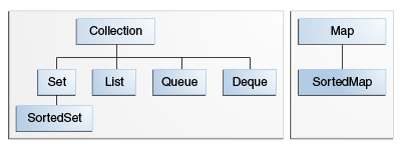
\includegraphics[width=4in]{colls-coreInterfaces.png}
\end{center}

\begin{itemize}
\item A {\it collection} is an object that represents a group of objects.
\item The collections framework allows different kinds of collections to be dealt with in an implementation-independent manner.
\end{itemize}


\end{frame}
%------------------------------------------------------------------------

%------------------------------------------------------------------------
\begin{frame}[fragile]{Collection Framework Components}

The Java collections framework consists of:
\begin{itemize}
\item Collection interfaces representing different types of collections (sets, lists, etc)
\item General purpose implementations (like {\tt ArrayList} or {\tt HashSet})
\item Absract implementations to support custom implementations
\item Algorithms defined in static utility methods that operate on collections (like {\tt Collections.sort(List<T> list)})
\item Infrastructure interfaces that support collections (like {\tt Iterator})
\end{itemize}
Today we'll learn a few basic concepts, then tour the collections library.
\end{frame}
%------------------------------------------------------------------------

%------------------------------------------------------------------------
\begin{frame}[fragile]{The {\tt Collection} Interface}


{\tt Collection} is the root interface of the collections framework, declaring basic operations such as:
\begin{itemize}
\item {\tt add(E e)} to add elements to the collection
\item {\tt contains(Object key)} to determine whether the collection contains {\tt key}
\item {\tt isEmpty()} to test the collection for emptiness
\item {\tt iterator()} to get an interator over the elements of the collection
\item {\tt remove(Object o)} to remove a single instance of {\tt o} from the collection, if present
\item {\tt size()} to find out the number of elements in the collection
\end{itemize}
None of the collection implementations in the Java library implement {\tt Collection} directly.  Instead they implement {\tt List} or {\tt Set}.

\end{frame}
%------------------------------------------------------------------------


%------------------------------------------------------------------------
\begin{frame}[fragile]{Lists and {\tt ArrayList}}
\vspace{-.05in}
The {\tt List} interface represents ordered collections, or {\it sequences}.  {\tt List} adds
\vspace{-.05in}  
\begin{itemize}
\item methods for positional (indexed) access to elements ({\tt get(int index)}, {\tt indexOf(Object o)}, {\tt remove(int index)}, {\tt set(int index, E element)}), 
\item a special iterator, {\tt ListIterator}, that allows element insertion and replacement, and bidirectional access in addition to the normal operations that the Iterator interface provides; and methods to obtain a {\tt ListIterator}
\item a {\tt subList(int fromIndex, int toIndex)} that returns a view of a portion of the list.
\end{itemize}
{\tt ArralyList} and {\tt LinkedList} are the two basic {\tt List} implementations provided in the Java standard library.\footnote{{\tt Vector} also implements {\tt List} and can be thought of as a synchronized version of {\tt ArrayList}.  You don't need {\tt Vector} if you're not writing multithreaded code.  Using {\tt Vector} in single-threaded code will decrease performance.}
\end{frame}
%------------------------------------------------------------------------

%------------------------------------------------------------------------
\begin{frame}[fragile]{{\tt ArrayList} Basics}


Create an {\tt ArrayList} with operator {\tt new}:
\begin{lstlisting}[language=Java]
  ArrayList tasks = new ArrayList();
\end{lstlisting}
Add items with {\tt add()}:
\begin{lstlisting}[language=Java]
  tasks.add("Eat");
  tasks.add("Sleep");
  tasks.add("Code");
\end{lstlisting}
Traverse with for-each loop:
\begin{lstlisting}[language=Java]
  for (Object task: tasks) {
      System.out.println(task);
  }
\end{lstlisting}

Note that the for-each loop implicitly uses an iterator.

\end{frame}
%------------------------------------------------------------------------

%------------------------------------------------------------------------
\begin{frame}[fragile]{Iterators}


Iterators are objects that provide access to the elements in a collection.  In Java iterators are represented by the {\tt Iterator} interface, which contains three methods:
\begin{itemize}
\item {\tt hasNext()} returns true if the iteration has more elements.
\item {\tt next()} returns the next element in the iteration.
\item {\tt remove()} removes from the underlying collection the last element returned by the iterator (optional operation).
\end{itemize}

The most basic and common use of an iterator is to traverse a collection (visit all the elements in a collection):
\begin{lstlisting}[language=Java]
ArrayList tasks = new ArrayList();
// ...
Iterator tasksIter = tasks.iterator();
while (tasksIter.hasNext()) {
    Object task = tasksIter.next();
    System.out.println(task);
}
\end{lstlisting}
See \link{\code/ArrayListBasics.java}{ArrayListBasics.java} for more.

\end{frame}
%------------------------------------------------------------------------

%------------------------------------------------------------------------
\begin{frame}[fragile]{Generics}


Did you notice the warning when we compile {\tt ArrayListBasics.java}?
\begin{lstlisting}[language=bash]
$ javac ArrayListBasics.java
Note: ArrayListBasics.java uses unchecked or unsafe operations.
Note: Recompile with -Xlint:unchecked for details.
\end{lstlisting}
% $
Java issues this warning because {\tt ArrayList} (and the other collecttion classes in the Java library) is a {\it parameterized type} and we used {\tt ArrayList} without a type parameter.  The full class name is {\tt ArrayList<E>}.
\begin{itemize}
\item {\tt E} is a {\it type parameter}, which can be any class name (not a primitive type).
\item {\tt ArrayList<E>} is a {\it parameterized type} 
\item {\tt E} tells the compiler which types are stored in the collection.
\end{itemize}
So the compiler is warning us that we're not using the type parameter and thus missing out on static type-checking.

\end{frame}
%------------------------------------------------------------------------

%------------------------------------------------------------------------
\begin{frame}[fragile]{Using Generics}


Supply a type argument in the angle brackets.  Read {\tt ArrayList<String>} as ``ArrayList of String''
\begin{lstlisting}[language=Java]
  ArrayList<String> strings = new ArrayList<String>();
  strings.add("Helluva"); strings.add("Engineer!");
\end{lstlisting}
If we try to add an object that isn't a {\tt String}, we get a compile error:
\begin{lstlisting}[language=Java]
  Integer BULL_DOG = Integer.MIN_VALUE;
  strings.add(BULL_DOG); // Won't compile
\end{lstlisting}

With a typed collection, we get autoboxing on insertion {\it and} retrieval:

\begin{lstlisting}[language=Java]
  ArrayList<Integer> ints = new ArrayList<>();
  ints.add(42);
  int num = ints.get(0);
\end{lstlisting}
Notice that we didn't need to supply the type parameter in the creation expression above.  Java inferred the type parameter from the declaration. (Note: this only works in Java 7 and above.)

See \link{\code/ArrayListGenericsDemo.java}{ArrayListGenericsDemo.java} for more.

\end{frame}
%------------------------------------------------------------------------

%------------------------------------------------------------------------
\begin{frame}[fragile]{Primitives in Collections}

{\tt ArrayList}s can only hold reference types.  So you must use wrapper classes for primitives:
\begin{lstlisting}[language=Java]
  ArrayList ints = new ArrayList();
  ints.add(new Integer(42));
\end{lstlisting}
Java auto-boxes primitives when adding to a collection:
\begin{lstlisting}[language=Java]
  ints.add(99);
\end{lstlisting}
But auto-unboxing can't be done when retrieving from an untyped collection:
\begin{lstlisting}[language=Java]
  int num = ints.get(0); // won't compile
\end{lstlisting}
The old way to handle this with untyped collections is to cast it:
\begin{lstlisting}[language=Java]
int num = (Integer) ints.get(0); // auto-unboxing on assignment to int
\end{lstlisting}

See \link{\code/ArrayListPrimitivesDemo.java}{ArrayListPrimitivesDemo.java} for more.
\end{frame}
%------------------------------------------------------------------------

%------------------------------------------------------------------------
\begin{frame}[fragile]{{\tt Set}s}

A {\tt Set} is a collection with no duplicate elements (no two elements {\tt e1} and {\tt e2} for which {\tt e1.equals(e2)}) and in no particular order.  Given:
\begin{lstlisting}[language=Java]
List<String> nameList = Arrays.asList("Alan", "Ada", "Alan");
Set<String> nameSet = new HashSet<>(nameList);
System.out.println("nameSet: " + nameSet);
\end{lstlisting}
will print:
\begin{lstlisting}[language=Java]
nameSet: [Alan, Ada]
\end{lstlisting}

\end{frame}
%------------------------------------------------------------------------

%------------------------------------------------------------------------
\begin{frame}[fragile]{{\tt Map}s}
\vspace{-.05in}
A {\tt Map<K, V>} is an object that maps keys of type {\tt K} to values of type {\tt V}.  The code:
\begin{lstlisting}[language=Java]
  Map<String, String> capitals = new HashMap<>();
  capitals.put("Georgia", "Atlanta");
  capitals.put("Alabama", "Montgomery");
  capitals.put("Florida", "Tallahassee");
  for (String state: capitals.keySet()) {
      System.out.println("Capital of " + state + " is "
                         + capitals.get(state));
  }
\end{lstlisting}
prints:
\vspace{-.05in}
\begin{lstlisting}[language=Java]
Capital of Georgia is Atlanta
Capital of Florida is Tallahassee
Capital of Alabama is Montgomery
\end{lstlisting}
\vspace{-.05in}
Note that the order of the keys differs from the order in which we added them.  The keys of a map are a {\tt Set}, so there can be no duplicates and order is not guaranteed.  If you {\tt put} a new value with the same key as an entry already in the map, that entry is overwritten with the new one.

\end{frame}
%------------------------------------------------------------------------


%------------------------------------------------------------------------
\begin{frame}[fragile]{Programming Exercise}

Write a class called {\tt WordCount}.
\begin{itemize}
\item The constructor should take a {\tt String} file name.
\item {\tt WordCount} should have an instance variable {\tt wordCounts} which is a {\tt Map} from {\tt String} to {\tt int}, where each {\tt String} key is a word that occurs in the file supplied to the constructor, and the corresponding {\tt int} is the number of times the word appears in the file.
\end{itemize}
Extra: normalize the word counts to $[0, 1]$ so that the word counts represent the probability that a randomly chosen word from the file is a given word.  For normalized word counts, what will be the type of the value in the map?
\end{frame}
%------------------------------------------------------------------------


% %------------------------------------------------------------------------
% \begin{frame}[fragile]{}


% \begin{lstlisting}[language=Java]

% \end{lstlisting}

% \begin{itemize}
% \item
% \end{itemize}


% \end{frame}
% %------------------------------------------------------------------------


\end{document}
